%%%%%%%%%%%%%%%%%%%%%%%%%%%%%%%%%%%%%%%%%%%%%%%%%%%%%%%%%%%%%%%%%%%%%%%
%%%                           SECTION III
%%%%%%%%%%%%%%%%%%%%%%%%%%%%%%%%%%%%%%%%%%%%%%%%%%%%%%%%%%%%%%%%%%%%%%

\chapter{\uppercase {Antisense mediated alternative splicing regulates imprinting of} \emph{Ube3a} \uppercase{in neurons}}

\subsubsection*{Abstract}

Loss of the maternally inherited \textit{UBE3A} allele causes Angelman syndrome, a debilitating neurological disorder associated with intellectual disability, absent speech, and ataxia.  In both mouse and human, the \textit{UBE3A} gene is imprinted with maternal-allelic expression in neurons of the CNS through the expression of the \textit{UBE3A} antisense transcript (\textit{UBE3A-AS}), which is both necessary and sufficient for establishing the imprint.  Unlike most imprinted genes though, \textit{UBE3A-AS} inhibits transcriptional elongation - rather than transcriptional initiation - of the paternal \textit{UBE3A} allele.  The mechanism by which this occurs is unknown.  Here we show that mouse \textit{Ube3a-AS} imprints \textit{Ube3a} through alternative splicing and the use of an intronic alternative polyadenylation site.  These findings provide insight into the functional significance of imprinting of \textit{UBE3A} in neurons and also reveal novel strategies to reactivate expression of the paternal \textit{UBE3A} as a therapy for individuals with Angelman syndrome. 

\section{Introduction}

Human chromosome 15q11-q13 contains a cluster of imprinted genes that are associated with number of neurogenetic syndromes. Maternal derived mutations or epimutations leading to the loss of ubiquitin protein ligase E3A (UBE3A) gene cause Angelman syndrome, which is associated with intellectual disability, ataxia, epilepsy, and an atypical happy disposition \cite{Matsuura1997,Kishino1997}. UBE3A is a member of the ubiquitin proteasome system, where it covalently attaches ubiquitin polypeptides to target proteins \cite{Scheffner1993}; it also functions as a co-activator of nuclear steroid hormone receptors \cite{Dhananjayan2006,Khan2006}. The specific targets and pathways underlying the symptoms associated with AS, however, remain unclear.  Paternal derived mutations or epimutations leading to the loss of the C/D box \textit{SNORD116} snoRNAs (small nucleolar RNAs) cause Prader-Willi syndrome (PWS), which is characterized by dysregulated hunger and satiety, thermoregulation, sleep-disorder, and behavioral issues \cite{Sahoo2008}.  Currently, the function of the \textit{SNORD116} snoRNAs in brain is poorly understood.

The \textit{UBE3A} gene is located at the telomeric end of the 15q11-q13 imprinted region and is orientated in the opposite direction of the C/D box snoRNA clusters (\textit{SNORD115} and \textit{SNORD116}) and the \textit{SNURF-SNRPN} gene.  The \textit{SNURF-SNRPN} gene and snoRNA clusters are expressed from the paternal allele as a long polycistronic transcriptional unit (PTU) that is also transcribed in the antisense direction across \textit{UBE3A} - the 3' end of the PTU is hence referred to as the \textit{UBE3A} antisense (\textit{UBE3A-AS}, also known as \textit{UBE3A-ATS}) transcript \cite{Runte2001}. Recent studies have demonstrated that transcription of \textit{UBE3A-AS} is both necessary and sufficient to silence expression of the \textit{UBE3A} sense transcript in mice \cite{Meng2013,Martins-Taylor2014}.  Moreover, since the PTU is transcribed exclusively from the paternal allele and expressed only in neurons, \textit{UBE3A} is imprinted with maternal-allelic expression in neurons and biallelically expressed in all other cell types \cite{Runte2001,Yamasaki2003}. An orthologous region exists on mouse chromosome 7C where imprinting of \textit{Ube3a} and the PTU is also conserved, which makes the mouse an excellent model for investigating the imprinting of \textit{Ube3a}.

Currently, the mechanism by which \textit{Ube3a-AS} inhibits expression of \textit{Ube3a} is unclear. Whereas most antisense transcripts regulate expression of their sense counterparts by inhibiting transcriptional initiation \cite{Latos2012,Umlauf2004,Williamson2011}, \textit{Ube3a-AS} appears to inhibit transcriptional elongation of \textit{Ube3a}. Meng \textit{et al.} \cite{Meng2013} reported that the paternal \textit{Ube3a} allele is modified with active histone modifications, bound by RNA polymerase II, and transcribed upto a region in intron 4, where both \textit{Ube3a} sense and antisense transcript levels diminish \cite{Meng2012,Numata2011}.  Based on these observations, Meng \textit{et al.} \cite{Meng2013} proposed a transcriptional collision model of genomic imprinting in which the \textit{Ube3a} and \textit{Ube3a-AS} transcriptional complexes collide, causing each to stall and dissociate from their respective template strands \cite{Meng2013}.

Recently, our laboratory detected high levels of \textit{Ube3a-AS} transcripts as far as 40 kb upstream of \textit{Ube3a} (\textbf{Chapter \ref{chapter2}}), which is at odds with the transcriptional collision model.  Based on this observation, we explored alternative mechanisms by which the antisense could inhibit transcriptional elongation of the paternal \textit{Ube3a} allele. Here, we demonstrate the existence of a paternally expressed, short \textit{Ube3a} isoform (isoform 4) that undergoes early termination through the use of an intronic alternative polyadenylation site in intron 4.  Isoform 4 is polyadenylated and expressed exclusively in the brain from the paternal allele. Pharmacological inhibition of \textit{Ube3a-AS} in mouse primary hippocampal neurons ablates the use of the intronic alternative polyadenylation site, resulting in reactivation of the paternal \textit{Ube3a} allele.  Based on these findings, we propose that \textit{Ube3a-AS} regulates imprinting of \textit{Ube3a} through alternative splicing and intronic alternative polyadenylation.

\section{Materials \& Methods}
\subsection{Bioinformatics}
\subsubsection{Public data, genomes and annotations}

\subsubsection*{Publicly available data}
The bioinformatic analysis performed in this chapter was conducted using publicly available data downloaded from the European Nucleotide Archive. Mouse tissue data was from 8 wk adults \cite{Pervouchine2015}. Topotecan treated neuron data were cultured cortical neurons (10 days \textit{in vitro}) with a 72 h treatment on day 7 \cite{King2013}. Finally, mouse cerebral cortex cellular populations data were purified using various methods specific to the cell-type \cite{Zhang2014}. A breakdown of tissue types, strain, and accession is supplied in \textbf{APPENDIX C, Table \ref{tableC:1}}. A complete list of publicly available RNA-seq datasets used in this chapter is provided in \textbf{Table \ref{public data:chp3}}. 

%%%%%%%%%%%%%%%%%%%%%%%%%%%%%%%%%%%%%%%%%%%%%%%%%%%%%%
\begin{longtabu} {X[.8,c]X[2,c]X[0.5,c]X[0.6,c]X[1.7,c]}
  \caption{Public Data: RNA-seq information for \textit{Ube3a} mechanism}\\
  \label{public data:chp3}\\
  \toprule
  \textbf{Study} & \textbf{Instrument} & \textbf{Layout} & \textbf{Stranded} & \textbf{Strain}\\
  \midrule
  \endhead
  ERP000591 & Illumina Genome Analyzer & PE    & No  & C57BL/6J x DBA/2J\\
  SRP012040 & Illumina HiSeq 2000      & PE    & Yes & C57BL/6J\\
  SRP017966 & Illumina HiSeq 2000      & PE/SE & No  & C57BL/6J x CASTEi/J\\
  SRP033200 & Illumina HiSeq 2000      & PE    & No  & Multiple\\
  \bottomrule
\end{longtabu}
%%%%%%%%%%%%%%%%%%%%%%%%%%%%%%%%%%%%%%%%%%%%%%%%%%%%%%

\subsubsection*{Genomes and annotation sets}
Throughout this work, the July 2007 finished NCBI Build 37 mouse genome assembly \cite{Chinwalla2002} (mm9) was used. Annotations were collected from Illumina iGenomes collection, using the July 17, 2015 UCSC annotations \cite{Rosenbloom2014}.

\subsubsection*{PolyA-seq and CAGE-seq data}
PolyA-seq BED files \cite{Derti2012} were downloaded from UCSC, while CAGE-seq BED files \cite{Lizio2015} were downloaded from \url{http://fantom.gsc.riken.jp/5/datafiles/latest/extra/CAGE_peaks/}. The polyA sites clustered datasets and CAGE-seq peak files was separated with \texttt{awk} (Bash version 4.0) and viewed with IGV (version 2.3.90 \cite{Thorvaldsdottir2013,Robinson2011}).

\subsubsection{Data processing}
The quality of the fastq files were checked with FastQC \cite{Andrews_Fastqc} (version 0.11.5), followed by adapter and low quality (quality score $\leq$ 3) sequence trimming with Trimmomatics \cite{Bolger2014} (version 0.36). The TruSeq3-PE-2.fa adapter file from Trimmomatics adapter file was used for adapter cutting and a minimal length of 25 was set. Paired- and single-end trimmed reads were than aligned with Hisat2 \cite{Pertea2016,Kim2015} (version 2.0.4) to chromosome 7 (chr7) with the assistance of Hisat2 provided python scripts that extracted splice sites and exons from chr7. The SAM file were directly pipped into SAMtools \cite{Li2009} (version 1.3.1) to convert to BAM format (\texttt{samtools view}) and sorted (\texttt{samtools sort}). These files were merged (\texttt{samtools merge}) and indexed (\texttt{samtools index}) by biological replicas for viewing in IGV. StringTie \cite{Pertea2015,Pertea2016} (version 1.3.3) was used to assemble the sorted BAM files (unmerged). Individual annotation files for stranded, high-depth reads (SRP01204) was generated via \texttt{stringtie} using the \textit{de novo} method, and merged (\texttt{stringtie -{}-merge}) using FPKM threshold of 5, and isoform fraction of 0.05. This merged annotation file was used as a reference for the Rsubread \cite{Liao2013a} (version 1.24.1) function \texttt{featureCounts} \cite{Liao2013b} for downstream analysis.

\subsubsection{Data analysis}
\subsubsection*{Visual analysis}
All visualization was conducted with IGV. Novel transcript annotation (GTF) on the forward strand were visualized along with polyA-seq and CAGE-seq brain-specific annotations (BED). For \textit{Ube3a} specific visualization, potential transcripts were extracted using a combination of \texttt{awk} and \texttt{grep}. Sashimi plots - a utility within IGV - were used to visualize alternative splicing limited to the forward strand.

\subsubsection*{Differential expression analysis with edgeR}
The Bioconductor \cite{Anders2013,Huber2015} (version 3.4, R \cite{Rcite2016} version 3.3.2) package, edgeR \cite{Chen2014,Robinson2009} (version 3.16.5), was used to determine differential expression on the transcript and exon level. Read counts were generated with \texttt{featureCounts}, which was used to generate an edgeR \texttt{DGEList} object from count, group, and annotation information. Data was filtered (CPM $\ge$ 1, for 25\% of samples) and normalized (\texttt{calcNormFactors}) before the dispersion was estimated \cite{Chen2014,Phipson2016} and fitted to a negative binomial generalized log-linear model \cite{McCarthy2012}. Isoform/transcript and exon levels differential expression was statistically tested with \texttt{exactTest} \cite{Robinson2007b} for pairwise comparisons of group means and p-values were adjusted using Benjamini \& Hochberg method (FDR) \cite{BH_1995} with \texttt{topTags} \cite{Robinson2007b,Robinson2007a}.

\subsubsection*{SNP analysis}
Informative SNPs were extracted from hybrid mice (maternal, C57BL/6J and paternal, DBA/J2) via \texttt{samtools mpileup} and BCFtools (version 1.3.1) \texttt{bcftools call} and \texttt{bcftools view} on sorted, indexed, merged BAM files. A list of SNPs in the region was downloaded from the Mouse Genomes Project - Query SNPs \cite{Keane2011,Yalcin2011} and coordinates were converted from mm10 to mm9 using LiftOver - an UCSC tool (\url{http://genome.ucsc.edu/cgi-bin/hgLiftOver}). Region of interest, specified with the \texttt{-r} option for \texttt{samtools mpileup}, was chr7:66,439,800-66,808,000.

\subsection{Molecular}
\subsubsection{Animals}
Animals were housed under standard conditions in a pathogen-free mouse facility. All procedures performed according to NIH guidelines and approved by the Texas A\&M University Institutional Animal Care and Use Committee (IACUC). The laboratory of Dr. Arthur Beaudet generated and provided \textit{Ube3a$^{YFP}$} mouse model \cite{Dindot2008}.  B6D2F1 (100006) hybrid mice were obtained from the Jackson Laboratory (Bar Harbor, ME). The \textit{Ube3a$^{YFP}$} mice were maintained on C57BL/6J background (000664, The Jackson Laboratory).

\subsubsection{Primary neuronal culture}
This study involved the establishment of primary hippocampal neurons from the offspring of female wild-type, C57BL/6J, and male \textit{Ube3a$^{+/YFP}$} mice as previously described \cite{Kavalali1999} with slight modifications. Briefly, hippocampi were dissected from P0-P2 mice and held on ice in hibernate medium (A1247501, Life Technologies, Carlsbad, CA) supplemented with 2\% B27 (17504044, Life Technologies) during surgery. Neurons were dissociated by trypsin treatment (10 min at 37$^{\circ}$C and 600 rpm) using TrypLE (12604021, Life Technologies) and triturated with a glass Pasteur pipette in Neuron culture media consisting of Neuralbasal Media (21103049, Life Technologies) supplemented with 1\% GlutaMAX (35050061, Life Technologies), 1\% penicillin/streptomycin (15140122, Life Technologies), and 2\% B27. Neurons were plated on 6-well cell culture plates coated with poly-l-ornithine (P0421, Sigma-Aldrich, St. Louis, MO) and laminin (23017015, Life Technologies). Typical plating density was one animal per well in a 6-well plate with cultures maintained at 37$^{\circ}$C (95\% O$_2$, 5\% CO$_2$).

\subsubsection{3' Rapid amplification of cDNA ends analysis}
Total RNA was isolated from flash frozen cortex of adult 10-week old male C57BL/6J mice using TRIzol (15596018, Life Technologies) following the manufacturer's protocol. Gene specific primers (\textbf{APPENDIX C, Table \ref{primerList}}) were designed to perform 3' RACE using AUAP universal primer (18373019, Life Technologies) following the manufacturer's protocol. PCR amplicons were cloned using the TOPO TA cloning kit (K458001, Life Technologies) and sequenced at the Texas A\&M University Gene Technologies Laboratory. Sequences were visualized with IGV using the \texttt{BLAT} function and BED files were exported, binded together (\texttt{paste}, Bash), sorted (\texttt{sortBed}) and merged (\texttt{bedtools merge}) with BEDtools \cite{Quinlan2010} (version v2.25.0). The merged BED files were visualized together with polyA- and CAGE-seq data in IGV.

\subsubsection*{Gene structure analysis}
Gene structure prediction was performed using the GeneSeqer program \cite{Brendel2004}. Briefly, the genome annotation was converted to a FASTA file using \texttt{gffread -w} (\url{http://ccb.jhu.edu/software/stringtie/gff.shtml#gffread}). The Ube3a protein ESTs (expressed sequence tags) were downloaded from NCBI as FASTA files. Using the \texttt{GeneSeqer} command for mouse, the forward strand was analyzed with the protein EST library for the predicted \textit{Ube3a} isoform 4.

\subsubsection{Cell culture treatment with Topotecan}
Total RNA was isolated from \textit{Ube3a$^{+/YFP}$} cultured primary neurons using a PureLink kit (12183018A, Life Technologies). Topotecan hydrochloride (1672257, Sigma-Aldrich) was added to 3 ml total of Neuron culture media in 6-well plate (72 h treatment) at a final concentration of 300 nM in 1X TE buffer (12090015, Life Technologies).

\subsubsection{Reverse-transcription and quantitative PCR analysis}
Four month old B6D2F1 female mice were dissected and the lung, liver, kidneys, heart, ovaries, and cortex were flash frozen. RNA was isolated using TRIzol and treated with TURBO DNA-free kit (AM1907, Life Technologies). Complementary DNA was generated using SuperScript IV (18091050, Life Technologies) with oligo(dT) primers. RT-PCR was preformed on adult mouse tissues with forward primer for exon 4 and reverse primers for exon 4.1 and 5. SYBR-Green (11760500, Life Technologies) was used to assay mRNA expression level using the 7900HT Fast Real-Time PCR System (4351405, Applied Biosystems, Foster City, CA). Expression data were normalized using \textit{ActB} and neuron expression was normalized using \textit{Map2}. All primers listed in \textbf{APPENDIX C, Table \ref{primerList}}. Statistical significance for qPCR expression data was determined using two-way ANOVA calculated in R (\texttt{aov}). Post-hoc analysis was performed simultaneously using Tukey's HSD multiple comparison (\texttt{TukeyHSD}) with default parameters.

\subsection{Charts}
Charts generated in R using \texttt{ggplot2} and \texttt{pdf}, a \texttt{devtools} function.

\section{Results}
\subsection{Novel \textit{Ube3a} isoform 4 expressed exclusively from the brain}
While investigating the alternative splicing patterns of \textit{Ube3a} in publicly available RNA-sequencing (RNA-seq) data sets, we identified a novel \textit{Ube3a} isoform involving splicing between exon 4 and an unannotated exon (hereafter referred to as exon 4.1) in intron 4 (\textbf{Figure \ref{sense annotation}A}).  The novel splice site was detected exclusively in transcriptome assemblies of mouse brain and not in any other organ or tissue (\textbf{APPENDIX C, Figure \ref{sense tissue splicing}}) and downregulated in other tissues (\textbf{APPENDIX C, Figure \ref{sense tissue fold-change}}). Moreover, alternative splicing into exon 4.1 was only detected in neurons (\textbf{APPENDIX C, Figure \ref{sense celltype splicing}}) and the isoform downregulated in other cell-types (\textbf{APPENDIX C, Figure \ref{sense celltype fold-change}}). 3'RACE and Sanger sequencing demonstrated that exon 4.1 was a terminal exon, aligning with the polyA-seq polyadenylation signal (\textbf{Figure \ref{sense annotation}B}), and revealing an in-frame coding sequence preceding a stop codon (\textbf{Figure \ref{sense annotation}C}). RT-PCR analysis (polyA enriched RNA) showed that \textit{Ube3a} isoform 4 was expressed in adult mouse cortex but not heart, liver, kidney, and ovary (\textbf{Figure \ref{sense annotation}D}), confirming our RNA-seq analysis.  Altogether, these data demonstrate the expression of a novel \textit{Ube3a} isoform expressed in brain, hereafter referred to as \textit{Ube3a} isoform 4.

%%%%%%%%%%%%%%%%%%%%%%%%%%%%%%%%%%%%%%%%%%%%%%%%%%%%%%
\begin{sidewaysfigure}
  \centering
  \resizebox{\linewidth}{!}{
    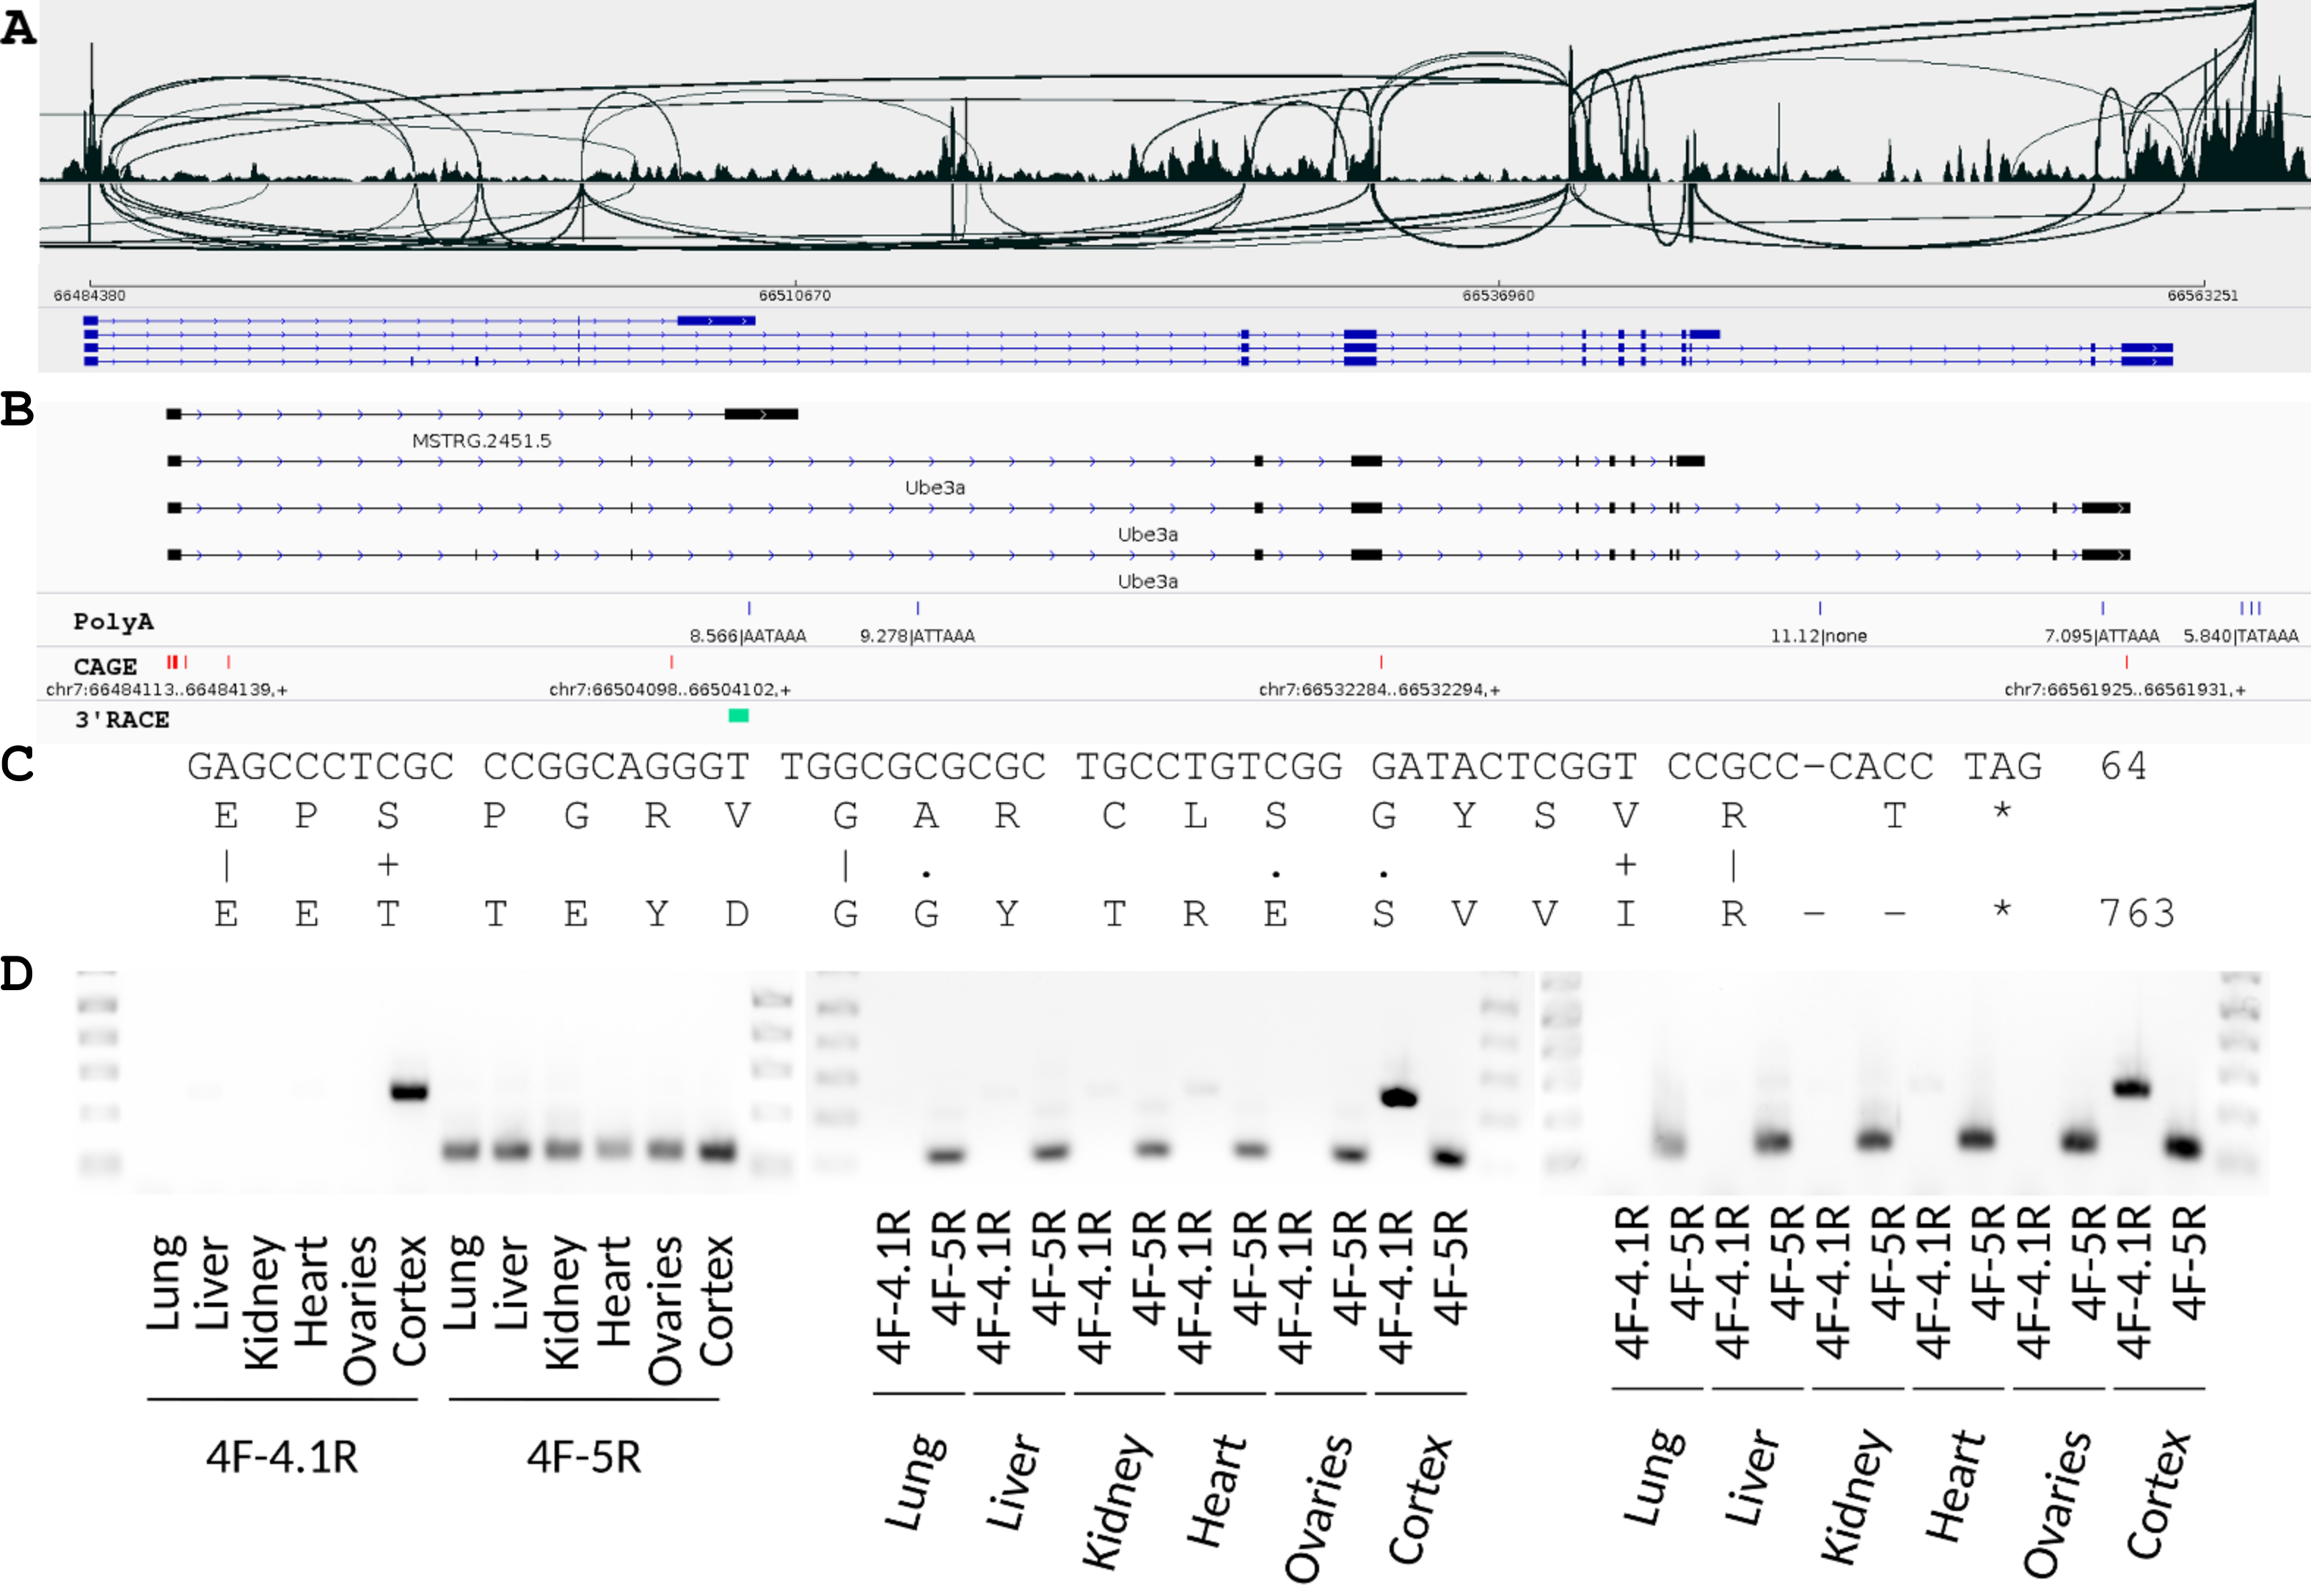
\includegraphics{figures/chapter3.fig1_short.png}
  }
  \caption{Identification of \textit{Ube3a} isoform 4 in mouse brain. \textbf{A.} Schematic of alternative splicing into \textit{Ube3a} exon 4.1 using merged cerebellum, cortex, and frontal lobe (n=2), stranded, paired-end RNA-seq data. Data generated from Pervouchine \textit{et al.} (2015). \textbf{B.} Schematic of alternatively spliced transcripts of \textit{Ube3a}. CAGE-seq 5' capping data produced by Lizio \textit{et al.} (2015). PolyA-seq data produced by Derti \textit{et al.} (2012). 3'RACE combined BLAT sequence \drawRACE[raceGreen]. \textbf{C.} Sequence alignment of \textit{Ube3a} exon 4.1 showing in-frame stop codon. \textbf{D.} RT-PCR showing that \textit{Ube3a} isoform 4 is exclusively expressed in the mouse brain.}
  \label{sense annotation}
\end{sidewaysfigure}
%%%%%%%%%%%%%%%%%%%%%%%%%%%%%%%%%%%%%%%%%%%%%%%%%%%%%%
\subsection{\textit{Ube3a} isoform 4 is paternally expressed}
We next investigated the mRNA (polyA enriched) transcriptomes of adult hybrid (C57BL/6J x DBA/2J) mice hippocampus (n = 6) produced by the Sanger Institute to determine the allelic expression of \textit{Ube3a} isoform 4. Analysis of informative single nucleotide variants (sense expressed transcripts) showed that \textit{Ube3a} isoform 4 was primarily expressed from the paternal allele (\textbf{Table \ref{snp freq}}, and \textbf{APPENDIX C, Figure \ref{informative snps}}).

%%%%%%%%%%%%%%%%%%%%%%%%%%%%%%%%%%%%%%%%%%%%%%%%%%%%%%%%
\begin{longtabu} {X[0.7,c]X[1.2,c]X[0.6,c]X[0.6,c]X[1,c]}
  \caption{SNP frequency for C57xDBA hybrid mice - exon 4.1 region}\\
  \label{snp freq}\\
  \toprule
  \textbf{SNP} & \textbf{Location} & \textbf{Ref} & \textbf{Alt} & \textbf{Allelic Freq}\\
  \midrule
  \endhead
  T/G & Chr7:66507227 & 0 & 7  & -1.00 \\
  C/T & Chr7:66508429 & 1 & 13 & -0.93 \\
  C/A & Chr7:66508469 & 1 & 30 & -0.96 \\
  G/A & Chr7:66509079 & 0 & 13 & -1.00 \\
  A/T & Chr7:66509131 & 0 & 17 & -1.00 \\
  \bottomrule
\end{longtabu}
%%%%%%%%%%%%%%%%%%%%%%%%%%%%%%%%%%%%%%%%%%%%%%%%%%%%%%
\subsection{\textit{Ube3a-AS} regulates the expression of \textit{Ube3a} isoform 4}
Our findings prompted us to hypothesize that the antisense transcript of \textit{Ube3a} regulated alternative splicing of \textit{Ube3a} isoform 4.  To test this, we first analyzed RNA-seq data generated by King \textit{et al.}, (2013), which consists of transcriptomes of mouse primary neurons treated either with a vehicle (DMSO) or Topotecan, a topoisomerase inhibitor that reactivates expression of the paternal \textit{Ube3a} allele by inhibiting expression of the \textit{Ube3a-AS} transcript \cite{King2013,Huang2012}.  Analysis of the transcriptomes revealed splicing into exon 4.1 in the control neurons but not the Topotecan treated neurons (\textbf{Figure \ref{topotecan treated neurons}A}). Analysis of isoform expression demonstrated significant downregulation of \textit{Ube3a} isoform 4 in Topotecan treated neurons; however, there did not appear to be a significant fold-change in expression of the other three isoforms (\textbf{Figure \ref{topotecan treated neurons}B}). 

An investigation into exon usage of \textit{Ube3a} showed similar expression levels of \textit{Ube3a} exon 4 in the control and Topotecan treated neurons; however, expression of exons 5 was significantly upregulated in the Topotecan treated neurons (\textbf{Figure \ref{topotecan treated neurons}C}), while it was significantly downregulated in exon 4.1. We then treated primary hippocampal neurons with Topotecan and vehicle (1X TE buffer) and used qPCR to quantify expression of \textit{Ube3a} isoform 4.  Consistent with the RNA-seq analysis, the Topotecan treated neurons had significantly reduced relative expression levels of \textit{Ube3a-AS} (TukeyHSD, p-value $<$ 0.0001) and \textit{Ube3a} isoform 4 (TukeyHSD, p-value $<$ 0.001) compared to controls (\textbf{Figure \ref{topotecan treated neurons}D}). Taken together these findings demonstrate that \textit{Ube3a-AS} regulates alternative splicing of \textit{Ube3a} paternal sense expression.

%%%%%%%%%%%%%%%%%%%%%%%%%%%%%%%%%%%%%%%%%%%%%%%%%%%%%%
\begin{sidewaysfigure}
  \centering
  \resizebox{\linewidth}{!}{
    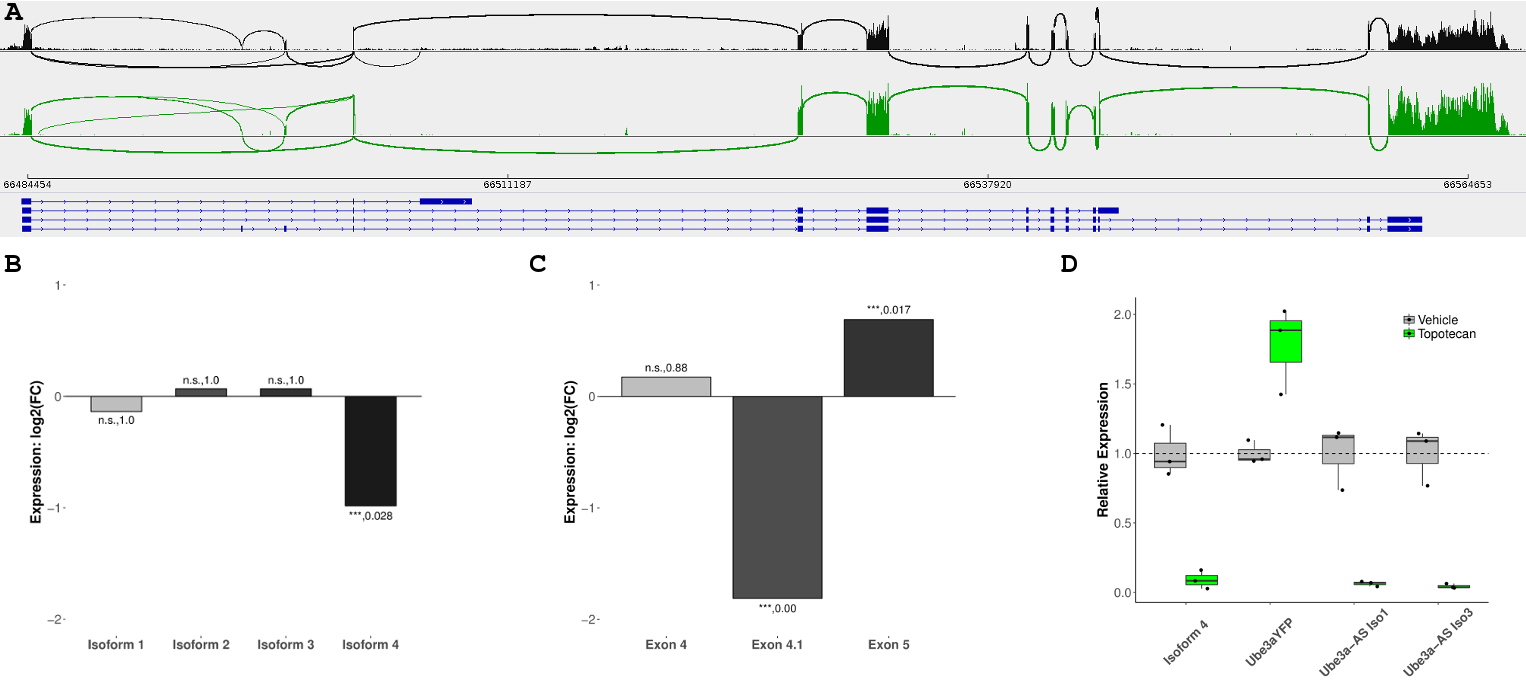
\includegraphics{figures/chapter3.fig2.png}
  }
  \caption{\textit{Ube3a-AS} regulates expression of \textit{Ube3a} isoform 4 in neurons. \textbf{A.} Schematic of \textit{Ube3a} splicing events detected by RNA-seq in primary neurons treated with vehicle (DMSO) and Topotecan (300 nM) for 72 h. Data generated from King \textit{et al.} (2013). \textbf{B.} Log2 fold-changed normalized expression of the four \textit{Ube3a} isoforms comparing Topotecan to vehicle treated neurons. \textbf{C.} Log2 fold-change of exons 4, 4.1, and 5 comparing Topotecan to vehicle treated neurons. \textbf{D.} \textit{Ube3a} isoform 4 and \textit{Ube3a-AS} relative expression levels in primary neurons treated with vehicle (1X TE buffer) and Topotecan (300 nM) (n = 3). P-value and FDR plotted in \textbf{B} and \textbf{C}. *** denotes p-value $<$ 0.001.}
  \label{topotecan treated neurons}
\end{sidewaysfigure}
%%%%%%%%%%%%%%%%%%%%%%%%%%%%%%%%%%%%%%%%%%%%%%%%%%%%%%

\section{Discussion}

Here we demonstrate the existence of a brain-specific, paternally expressed \textit{Ube3a} isoform that terminates in intron 4 and that is dependent on expression of the \textit{Ube3a-AS} transcript.  Based on these findings, we propose that \textit{Ube3a-AS} inhibits transcriptional elongation of the paternal \textit{Ube3a} allele through alternative splicing and the use of an intronic alternative polyadenylation signal.  This notion is consistent with numerous reports, including imprinted genes, describing the antisense regulation of sense alternative splicing \cite{MacIsaac2011,Morrissy2011}.  Whether transcription of \textit{Ube3a-AS} affects the elongation kinetics of the paternal \textit{Ube3a} transcriptional complex, leading to inclusion of the exon 4.1, or whether the \textit{Ube3a-AS} transcript induces inclusion of exon 4.1 by masking the downstream splice acceptor sites or regulatory elements is unknown and warrants further investigation.

We investigated the link between \textit{Ube3a-AS} and \textit{Ube3a} isoform 4 with Topotecan, a drug known to effect alternative splicing \cite{Shkreta2008,Powell2013b}; and thus, this study does not clarify whether the reduction in \textit{Ube3a} isoform 4 expression is due primarily to the decrease in \textit{Ube3a-AS} expression or due to Topotecan. An alternative method to inhibition \textit{Ube3a-AS} specifically with either antisense oligonucleotides, similar to Meng \textit{et al.} (2013), or by using a PWS-IC paternal deletion transgenetic mouse model would answer this question. Nevertheless, we provide for the first time evidence linking \textit{Ube3a-AS} expression to alternative splicing of the paternal \textit{Ube3a} sense transcript.

Based on our findings, we envision at least three scenarios that could explain the functional significance of \textit{UBE3A} imprinting in neurons. First, isoform 4 may have a neuron-specific regulatory role. In this model, the expression of the antisense transcript expands the functionality of \textit{Ube3a} specifically in neurons.
This theory is further supported by our results showing temporal regulation of isoform 4 in hippocampal tissue (\textbf{APPENDIX C, Figure \ref{temporal sense expression}}).
Conversely, the antisense transcript may have neuron-specific regulatory functions. Given the recent studies in our laboratory demonstrating a remarkable complexity to \textit{Ube3a-AS/UBE3A-AS} expression patterns, with more than a dozen alternatively spliced transcripts in mouse and at least ten alternatively spliced transripts in human, suggests a regulatory role for \textit{Ube3a-AS/UBE3A-AS} in the brain (\textbf{Chapter \ref{chapter2}}). Although the functionality of these transcripts has yet to be investigation, their existence suggests a model in which reciprocal imprinting allows for the expression of both sense and antisense transcripts (i.e., the complementation model) \cite{Kaneko-Ishino2006,Kaneko-Ishino2003}.
Finally, it is possible that both isoform 4 and the antisense transcripts have a regulatory role within the brain; and thus, increase the overall complexity of the treanscriptome in neurons.

In addition to proposing a new model for the imprinting of \textit{Ube3a} in neurons, these results also apply to the current therapeutic strategies for Angelman syndrome - reactivation of the paternal \textit{UBE3A} allele. Numerous laboratories, including ours, are actively pursuing strategies to reactive expression of the paternal \textit{Ube3a/UBE3A} allele. The feasibility of this approach has been demonstrated using both pharmacological and epigenetic methodologies \cite{Huang2012,Meng2015,Bailus2016}.  More importantly, reactivation of the paternal \textit{Ube3a} allele has been shown to mitigate some of the phenotypes associated with the loss of \textit{Ube3a} in an Angelman syndrome mouse model \cite{Meng2015,Shi2015}. The link between isoform 4 and reactivation of the paternal \textit{Ube3a} allele offers a new target for AS therapeutics. Furthermore, it highlights potential ramifications for the knockdown of \textit{Ube3a} isoform 4 and \textit{Ube3a-AS}.
